\documentclass{standalone}
\usepackage{graphicx}	
\usepackage{amssymb, amsmath, amsthm}
\usepackage{color}

\usepackage{tikz}
\usetikzlibrary{intersections, backgrounds}

\definecolor{light}{RGB}{220, 188, 188}
\definecolor{mid}{RGB}{185, 124, 124}
\definecolor{dark}{RGB}{143, 39, 39}
\definecolor{highlight}{RGB}{180, 31, 180}
\definecolor{gray10}{gray}{0.1}
\definecolor{gray20}{gray}{0.2}
\definecolor{gray30}{gray}{0.3}
\definecolor{gray40}{gray}{0.4}
\definecolor{gray60}{gray}{0.6}
\definecolor{gray70}{gray}{0.7}
\definecolor{gray80}{gray}{0.8}
\definecolor{gray90}{gray}{0.9}
\definecolor{gray95}{gray}{0.95}

\begin{document}

\begin{tikzpicture}[scale=0.4, thick]

\begin{scope}[shift={(0, 0)}]
    \draw[white] (-9.75, -7) rectangle (9.75, 7);
      
    \begin{scope}
      \clip (-7, -7) rectangle (7, 6);
          \node at (0, 0) {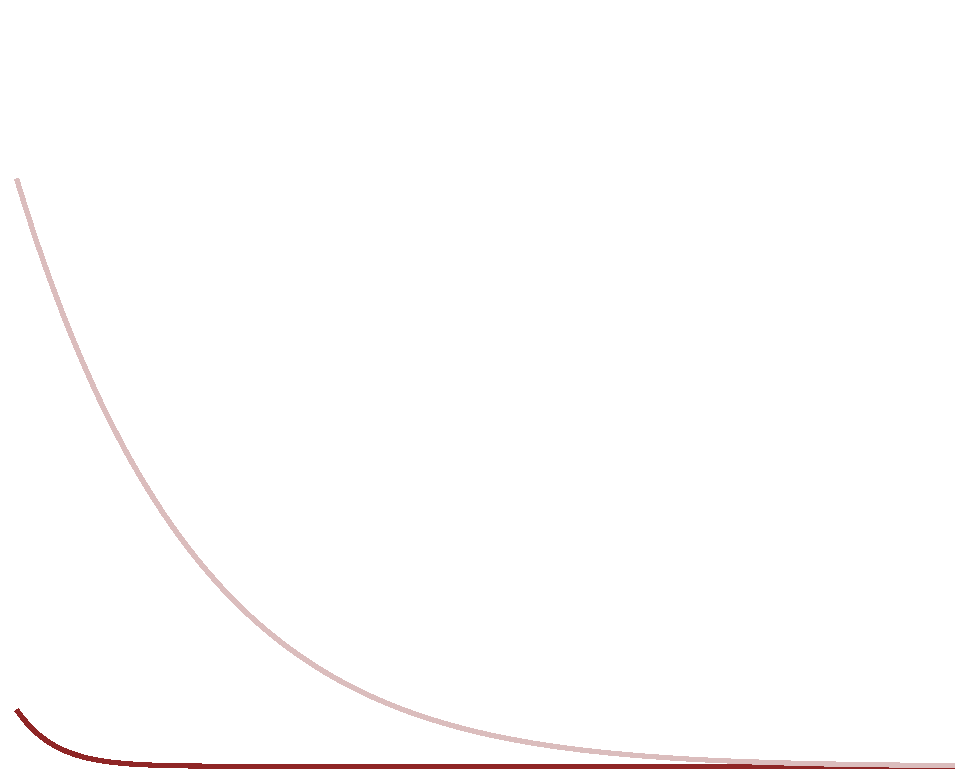
\includegraphics[height=4cm]{containment_zoom.eps}};
    \end{scope}
   
    
    \node[dark] at (0, -4) { Derived From Normal Prior };
    \node[light] at (1, 0) { Derived From Cauchy Prior };
    
    \draw [->, >=stealth, line width=1] (-6.22 - 0.035, -5) -- +(12.44, 0);
    \node at (0, -6) { $\theta$ };
    
    \draw [->, >=stealth, line width=1] (-6.22, -5 - 0.035) -- +(0, 11);
    \node[rotate=90, align=center] at (-8, 0) { Posterior Probability\\Distribution Function };

\end{scope}


\end{tikzpicture}

\end{document}  